% !TEX root = ../../main.tex

\section{Context and scientific approach}

Adsorption induced changes in porous media have been known
to occur for over 90 years~\cite{mcbainNatureInfluenceHumidity1927},
with both clays, coals and polymers undergoing swelling during gas
or vapour uptake~\cite{gorAdsorptioninducedDeformationNanoporous2017}.
In the case of clays, this change in volume is due to cleavage 
of weak hydrogen bonds leading to separation of layers. The 
mechanism is similar in the nanopores of bitumen-containing coal
and in polymers, with both mechanisms being driven by adsorption
induced stress. In-depth studies~\cite{beringAlterationZeoliteGranule1977} 
have revealed that most porous materials posses some small
degree of compliance, with \textit{in-situ }dilatometry going so far as to 
obtain pore size distributions from accurate volume
changes~\cite{reichenauerExtractingPoreSize2001}. This type of
swelling, contraction and expansion usually follows a second order
transition.

The discovery of similar types of compliant behaviour upon 
adsorption in metal organic frameworks has opened new perspectives 
in the area, as they have been shown to undergo massive and 
reversible structural deflections, while retaining their crystalinity.
Some of the known types of structural flexibility encountered in MOFs
is presented in \autoref{dut:fgr:flex-types}. 


\begin{figure}[htb]
    \centering
    
    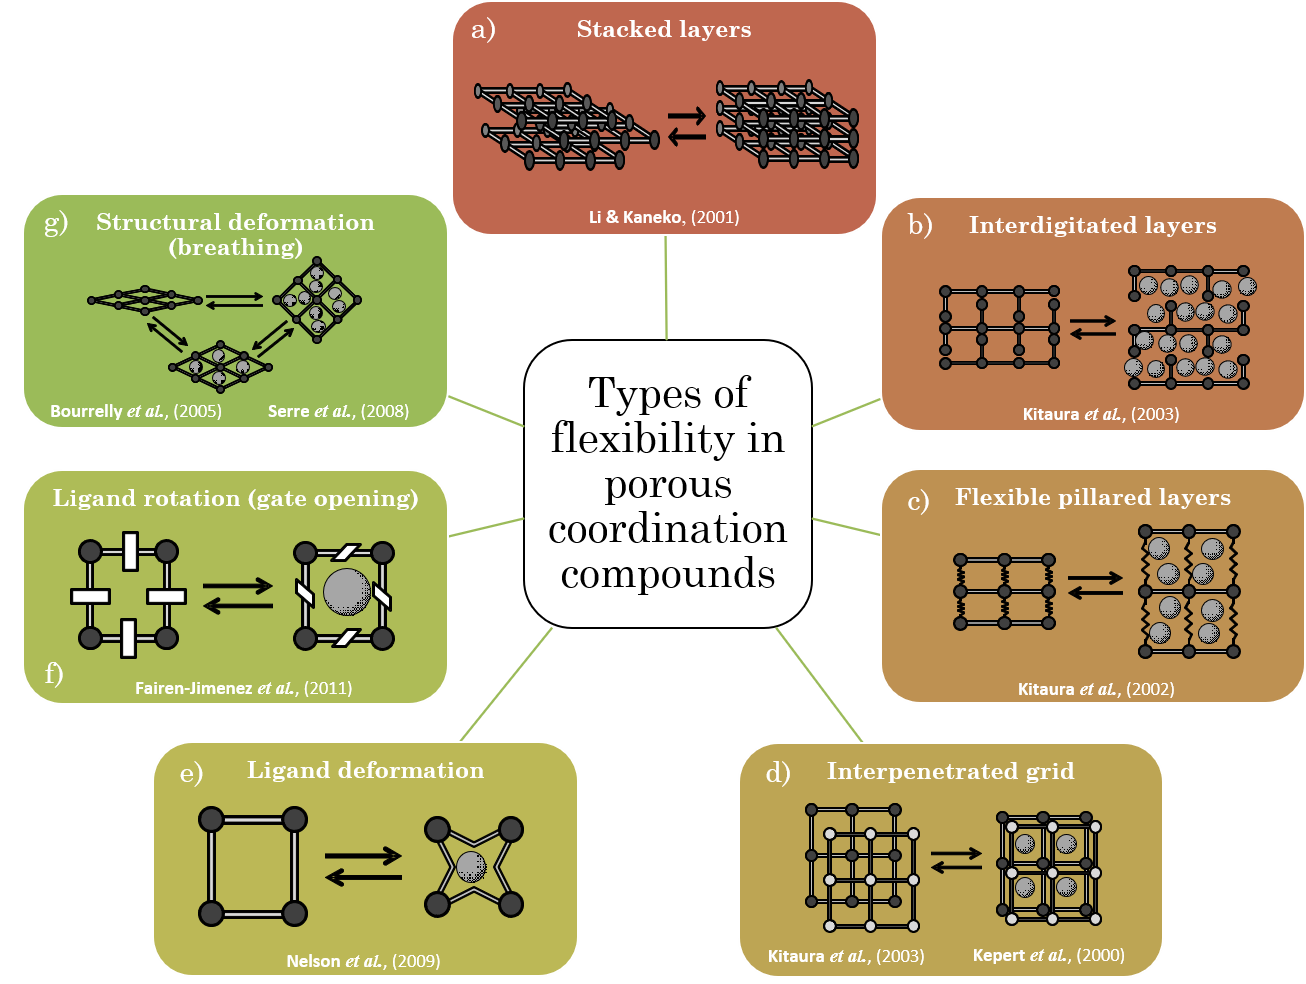
\includegraphics[width=\textwidth]{flexibility-types}%
    \caption{A visual summary of the types of flexibility
    which are documented in MOFs, as detailed in 
    (a)~\citet{liHydrogenBondregulatedMicroporous2001}
    (b)~\citet{kitauraPorousCoordinationPolymerCrystals2003}
    (c)~\citet{kitauraPillaredLayerCoordinationPolymer2002}
    (d)~\citet{kepertVersatileFamilyInterconvertible2000,%
    kitauraPorousCoordinationPolymerCrystals2003}
    (e)~\citet{nelsonSupercriticalProcessingRoute2009}
    (f)~\citet{fairen-jimenezOpeningGateFramework2011}
    (g)~\citet{bourrellyDifferentAdsorptionBehaviors2005, %
    serreExplanationVeryLarge2007}}%
    \label{dut:fgr:flex-types}
    
\end{figure}

The discovery of the so-called ``breathing'' type of structural
deformation in the MIL-53 family of materials has shown that 



Finding a suitable model that would predict such structural changes
has remained a challenge. A successful model for 
~\cite{neimarkStressBasedModelBreathing2010}
~\cite{gorAdsorptionInducedDeformationMesoporous2010}
Nevertheless a complete theory of adsorption-deformation 
which can fully predict the changes in the measured enthalpy of 
adsorption and the mechanistic behaviour of theoretical structures
has remained elusive.

The usefulness of such phenomena have been long recognised as potential
sensors or actuators, initially by nature itself, with humidity induced 
swelling acting to open pine cones~\cite{dawsonHowPineCones1997}. 
More recently similar sensing devices based on adsorption induced 
strain in mesoporous silica have been 
developed~\cite{boudotConvertingWaterAdsorption2016, %
ganserCantileverBendingBased2016} which show promise for use 
in micromechanical systems. From a gas storage and separation 
point of view, changes in the adsorbent structure may be crucial 
for process improvement. Pressure swing adsorption (PSA) is heavily 
dependent on the working capacity of the adsorbent used, or the
difference between loading at the operation pressure and at the 
regeneration pressure. In this case, an S-shaped isotherm, with 
the vertical part of the slope in the aforementioned pressure 
range would lead to high process efficiency gains by eliminating material
``dead volume adsorbed''. In a temperature swing process (TSA), where 
the regeneration is performed through heating of the adsorbent 
bed, the key parameter is the integral enthalpy of adsorption, a measure 
of the energy requirements for the process. As a part of the chemical 
potential of the adsorbed phase is used by the mechanical contraction
of the material, flexible adsorbents have the potential of
intrinsic thermal management, reducing the energy cost.
Finally, swelling of clays upon gas adsorption 
is quickly becoming a research interest as extraction of shale 
deposits is becoming common. In particular, the attractive option
of combined carbon capture and methane recovery implemented 
through pumping of carbon dioxide into reservoirs leads to swelling-induced
loss of porosity and well blocking due to the increased strain 
by \ce{CO2} in comparison to methane. 

However, the most promising perspective for such materials come from
